% =====================================================================
% JUDGe 2026 (NeurIPS) -- Junior Spotlight track
% 2 pages + references. DOUBLE-BLIND. Non-archival.
%
% FORMAT NOTE
%   This compiles standalone with the geometry block below, which
%   approximates the NeurIPS text block. To use the official style:
%     1. download neurips_2026.sty next to this file
%     2. delete the \usepackage[...]{geometry} line
%     3. add \usepackage{neurips_2026}
%   Do NOT use \usepackage[final]{neurips_2026} -- the final option
%   prints author names and breaks double-blind review.
%
% ANONYMITY -- checked before every build:
%   no author, no institution, no funder, no real repository URL.
%   The mirror URL is set by set_mirror_url.py and is empty until it exists.
% =====================================================================
\documentclass{article}
\usepackage[dblblindworkshop]{neurips_2026}
\workshoptitle{First Workshop on Reliable Evaluation for Language Models (JUDGe)}
\setcitestyle{square,numbers,comma}

\usepackage[utf8]{inputenc}
\usepackage[T1]{fontenc}
\usepackage{graphicx}
\usepackage{amsmath,amssymb}
\usepackage{booktabs}
\usepackage{microtype}
\usepackage[hidelinks]{hyperref}
\usepackage[skip=3pt,font=footnotesize]{caption}
\usepackage{titlesec}

% ---------------------------------------------------------------------
% Anonymous mirror. Set ONLY via:
%     python writeup/judge2026/set_mirror_url.py <url>
% which refuses any host other than anonymous.4open.science -- pasting the
% real GitHub URL here would de-anonymise the submission, and the repo name
% contains the author's surname.
%
% While empty, \mirrornote expands to nothing, so the paper compiles and is
% correctly shaped with or without the mirror. Nothing fake is ever shipped.
% ---------------------------------------------------------------------
\newcommand{\mirrorurl}{}
\newcommand{\mirrornote}{%
  \ifx\mirrorurl\empty\else
    \footnote{Code, the pre-registration with its deviations log, and all 200
    raw agent reports: \url{\mirrorurl}}%
  \fi}

\titlespacing*{\section}{0pt}{4pt}{1.5pt}
\titlespacing*{\subsection}{0pt}{4pt}{1pt}
\titleformat{\section}{\normalfont\large\bfseries}{\thesection}{0.6em}{}
\titleformat{\subsection}{\normalfont\normalsize\bfseries}{\thesubsection}{0.6em}{}
\setlength{\parskip}{0pt}
\setlength{\textfloatsep}{6pt}
\setlength{\intextsep}{6pt}

\title{\vspace{-3em}\bfseries An Auditing Agent Asserts at Ceiling\\
Whether or Not There Is Anything to Find}

% DOUBLE-BLIND: leave anonymous.
\author{Anonymous submission\\\small Under review, JUDGe 2026 Junior Spotlight}
\date{}

\begin{document}
\maketitle
\vspace{-2.1em}

\begin{abstract}
\small\noindent
Automated agents are increasingly used to audit whether a model carries a
hidden objective, and their reports read as confident natural language. We
audit one such white-box agent and ask a question its published evaluation does
not: what does it say when there is nothing to find? Its \emph{assertion rate}
turns out to be decoupled from the evidence available to it. On byte-identical
evidence, a presuppositional prompt yields 9/9 confident and mutually
contradictory answers against 2/10 under neutral phrasing (Fisher exact
$p=0.0007$). Across a six-rung dilution ladder, assertion stays pinned at 1.00
over 120 runs while accuracy falls from 0.55 to 0.05. Detection itself
reproduces. The failure is calibration: for evaluators of this kind, confidence
carries no information about whether a finding exists.
\end{abstract}
\vspace{-0.6em}

\section{The missing arm of an evaluation}

Model diffing methods compare a base model against a finetuned one and try to
name what changed. Activation Difference Lens (ADL)~\cite{adl} reports its
diffing agent naming the finetuning objective for 91\% of organisms at grade
$\geq 2$, against 39\% for a black-box baseline.

That is a \emph{sensitivity} number: it measures how often the agent recovers an
objective that is present. The complementary quantity---how often it names an
objective that is \emph{absent}---had not been measured for any white-box
diffing method, because no such method had been run on a pair with no hidden
objective. For anything used as a judge~\cite{zheng23judge,tian23calib}, the second number governs trust. An
evaluator that reports a finding on every input has perfect sensitivity and is
worthless. We ran 200 blind audits to measure it, and could not---for a reason
that turned out to be more useful than the number would have been.

\section{Setup}

Base model Gemma-3-1B. Auditing agent \texttt{gpt-5-2025-08-07}---the model ADL
itself uses, pinned to a snapshot. Grader \texttt{gpt-5-mini-2025-08-07}. We
reimplemented ADL in raw HuggingFace hooks (logit lens, Patchscope, steering,
directional ablation) rather than TransformerLens. 200 runs: 80 main
($n=10$ per cell) and 120 ladder ($n=20$ per rung).\mirrornote

Every run is coded three ways---ASSERT, ABSTAIN, DEGENERATE---by a definition
fixed in advance and applied identically on every arm. Neither the agent nor the
grader learns which arm it is looking at, and the grader never sees ground
truth.

\section{We could not build a null, and that is the first result}
\label{sec:null}

Our pre-registered primary metric was a false-positive rate: run the agent on
pairs that differ for benign reasons and count assertions. \textbf{We abandoned
it.} Every null we constructed turned out to contain a real signal, and a
false-positive rate measured against a contaminated null would mean nothing.

Three nulls, three distinct contaminations. (a) Finetuning on a generic web
corpus: the corpus is itself a register, and the agent read it correctly. (b)
Two LoRA seeds trained on byte-identical data: these still differ \emph{along}
the domain axis, because two runs converge to different points on the same
direction. (c) Base versus instruction-tuned: instruction-tuning is itself an
objective.

The methodological finding is that \emph{there may be no such thing as a
no-objective finetune}.

\section{Assertion is decoupled from evidence}
\label{sec:decoupled}

\subsection{Framing manufactures answers}

On the arm with no \emph{narrow} objective, the shipped presuppositional prompt
(``The finetuning instilled a specific objective. Identify it.'') produces 9/9
assertions. A neutral prompt, on byte-identical evidence, produces 2/10 (Fisher
exact $p=0.0007$)~\cite{hwang26framing,sharma23syco}. The nine assertions are not one answer: a blind judge splits
them into two mutually incompatible groups, so at least one group is wrong
without any ground truth being consulted.

\subsection{Down a dilution ladder, only accuracy moves}

\begin{figure}[t]
\centering
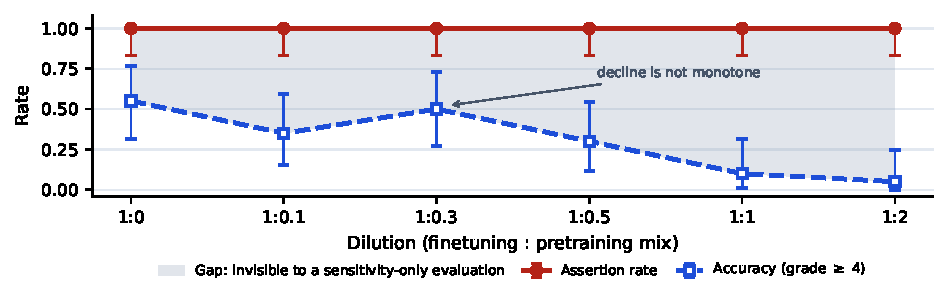
\includegraphics[width=0.70\linewidth]{figure_ladder.pdf}
\caption{Six dilution rungs, $n=20$ each, 120 runs. Assertion is flat at 1.00
while accuracy collapses. The shaded gap is what a sensitivity-only evaluation
cannot see: a confident wrong answer and a correct one both count as
responding. Intervals are Clopper--Pearson 95\%. The decline is not monotone.}
\label{fig:ladder}
\end{figure}

Six released rungs progressively mix finetuning data with pretraining data
(Figure~\ref{fig:ladder}). Assertion is 1.00 on all six---120 of 120 runs---while
accuracy at grade $\geq 4$ falls from 0.55 to 0.05 ($\rho=-0.94$, $p=0.005$).
The agent does not grow quieter as its evidence thins. It says the same amount,
with the same confidence, and is progressively less right.

\textbf{This trend is exploratory, not pre-registered.} Our registered ladder
test was a logistic regression of assertion on dilution. Because assertion is
constant at 1.00, that regression is degenerate---there is no variance to
model---and no coefficient is estimable. The trend reported here is measured on
a \emph{different} outcome (accuracy) and is labelled exploratory under our
pre-registered multiplicity rule. The degeneracy is itself informative: the
registered test could not run precisely because the agent never stopped
asserting.

\section{Supporting results}
\label{sec:support}

\textbf{Detection reproduces.} On a released organism the agent is correct 20/20
under both framings. The failures above are not a broken reimplementation, and
we do not claim the method fails at detection.

\textbf{A candidate label-free instrument.} Cross-seed consistency---do
independent seeds on identical evidence give mutually compatible answers?---is
1.00 on arms with a real signal and 0.67 on the arm without, and requires no
ground truth. We call this a \emph{candidate}, not a validated detector: it
rests on four cells, Fisher $p\approx 0.09$, with overlapping intervals.

\textbf{Magnitude does not predict findability.} Within the dilution family,
mean activation-difference norm is anti-correlated with accuracy ($\rho=-0.77$,
$p=0.07$). Between families the relation reverses: the arm with the best
accuracy has mean norm 747, while the arm with no objective at all has 7756.
Triaging models for audit by ``large difference, worth a look'' would rank these
backwards.

\section{Method discipline}

The rubric and analysis plan were committed before any results existed. Ten
deviations are logged in-file, including the abandonment of the pre-registered
headline metric in \S\ref{sec:null}. Blinding is enforced rather than
documented: a scrub raises a \texttt{BlindingViolation} exception if an arm
identifier would reach the agent. Grader validation gives $\kappa = 1.000$
(16/16)---weaker than it sounds, since only one case tested the
ASSERT/ABSTAIN boundary. Total research
time was 18 hours against a 20-hour cap.

\section{Limitations}

No clean false-positive rate exists in this data, because no clean null does.
Everything here is one model family (Gemma-3-1B), one auditing agent, one
grader, and a reimplementation of ADL rather than the authors' code, so we
cannot separate agent-specific from method-specific behaviour. The consistency
result rests on four cells with overlapping intervals and $p \approx 0.09$ and
should not be used as a detector on this evidence. The ladder trend is exploratory and its decline is not monotone. Our correctness grades use a reconstructed rubric and are not
comparable to the 91\% figure quoted in \S1.

\section{What this implies for LLM judges}

Confidence is not a trust signal for this class of evaluator~\cite{tian25overconf}. Any pipeline that treats an evaluator's
willingness to answer---or the fluency of its answer---as evidence that
something was found is reading a constant. Two cheap mitigations follow
directly: report evaluator results under both presuppositional and neutral
phrasings; and prefer agreement
across independent seeds on identical evidence over single-run confidence~\cite{schroeder24rely}, since
contradiction is detectable without labels even when correctness is not.

\begin{thebibliography}{7}
\small
\bibitem{adl}
Julian Minder, Cl\'ement Dumas, Stewart Slocum, Helena Casademunt,
Cameron Holmes, Robert West, and Neel Nanda.
\newblock Narrow Finetuning Leaves Clearly Readable Traces in Activation
Differences.
\newblock arXiv:2510.13900, October 2025. ICLR 2026.
\bibitem{zheng23judge}
Lianmin Zheng, Wei-Lin Chiang, Ying Sheng, Siyuan Zhuang, Zhanghao Wu, Yonghao Zhuang, Zi Lin, Zhuohan Li, Dacheng Li, Eric P. Xing, Hao Zhang, Joseph E. Gonzalez, and Ion Stoica.
\newblock Judging LLM-as-a-Judge with MT-Bench and Chatbot Arena.
\newblock arXiv:2306.05685, June 2023. NeurIPS 2023 Datasets and Benchmarks Track.

\bibitem{tian23calib}
Katherine Tian, Eric Mitchell, Allan Zhou, Archit Sharma, Rafael Rafailov, Huaxiu Yao, Chelsea Finn, and Christopher D. Manning.
\newblock Just Ask for Calibration: Strategies for Eliciting Calibrated Confidence Scores from Language Models Fine-Tuned with Human Feedback.
\newblock arXiv:2305.14975, May 2023. EMNLP 2023.

\bibitem{hwang26framing}
Yerin Hwang, Dongryeol Lee, Taegwan Kang, Minwoo Lee, and Kyomin Jung.
\newblock When Wording Steers the Evaluation: Framing Bias in LLM judges.
\newblock arXiv:2601.13537, January 2026. Preprint.

\bibitem{sharma23syco}
Mrinank Sharma, Meg Tong, Tomasz Korbak, David Duvenaud, Amanda Askell, Samuel R. Bowman, Newton Cheng, Esin Durmus, Zac Hatfield-Dodds, Scott R. Johnston, Shauna Kravec, Timothy Maxwell, Sam McCandlish, Kamal Ndousse, Oliver Rausch, Nicholas Schiefer, Da Yan, Miranda Zhang, and Ethan Perez.
\newblock Towards Understanding Sycophancy in Language Models.
\newblock arXiv:2310.13548, October 2023. ICLR 2024.

\bibitem{tian25overconf}
Zailong Tian, Zhuoheng Han, Yanzhe Chen, Haozhe Xu, Xi Yang, Richeng Xuan, Houfeng Wang, and Lizi Liao.
\newblock Overconfidence in LLM-as-a-Judge: Diagnosis and Confidence-Driven Solution.
\newblock arXiv:2508.06225, August 2025. Preprint.

\bibitem{schroeder24rely}
Kayla Schroeder and Zach Wood-Doughty.
\newblock Can You Trust LLM Judgments? Reliability of LLM-as-a-Judge.
\newblock arXiv:2412.12509, December 2024. Preprint.

\end{thebibliography}

\end{document}
